%%%%%%%%%%%%%%%%%%%%%%%%%%%%%%%%%%%%%%%%%%%%%%%%%%%%%%%%%%%%%%%%%%%%%%%%%%%%%%%%%%%%%%%%%%%%%%%%%%%%%%%%%%%%%%%%%%%%%%%%%%%%%%%%%%%%%%%%%%%%%%%%%%%%%%%%%%%%%%%%%%%
% Written By Michael Brodskiy
% Class: Fundamentals of Electronics
% Professor: I. Salama
%%%%%%%%%%%%%%%%%%%%%%%%%%%%%%%%%%%%%%%%%%%%%%%%%%%%%%%%%%%%%%%%%%%%%%%%%%%%%%%%%%%%%%%%%%%%%%%%%%%%%%%%%%%%%%%%%%%%%%%%%%%%%%%%%%%%%%%%%%%%%%%%%%%%%%%%%%%%%%%%%%%

\include{Includes.tex}

\title{Pre-Lab 1}
\date{\today}
\author{Michael Brodskiy\\ \small Professor: M. Onabajo}

\begin{document}

\maketitle

\begin{enumerate}

  \item Review section read \textcolor{green}{\checkmark}

  \item The power supplies can be connected as shown:

    \begin{figure}[H]
      \centering
      \tikzset{every picture/.style={line width=0.75pt}} %set default line width to 0.75pt        

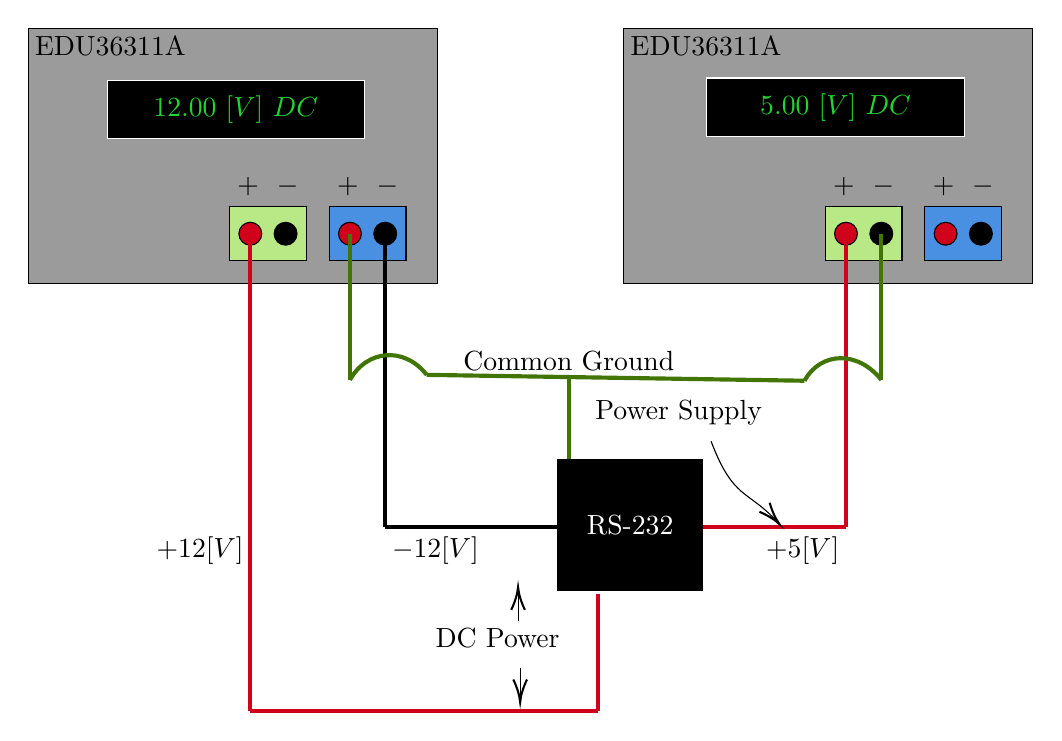
\begin{tikzpicture}[x=0.75pt,y=0.75pt,yscale=-1,xscale=1]
%uncomment if require: \path (0,437); %set diagram left start at 0, and has height of 437

%Shape: Rectangle [id:dp40376072703618315] 
\draw  [fill={rgb, 255:red, 155; green, 155; blue, 155 }  ,fill opacity=1 ] (43,81) -- (240,81) -- (240,204) -- (43,204) -- cycle ;
%Shape: Rectangle [id:dp9680918137452028] 
\draw  [fill={rgb, 255:red, 74; green, 144; blue, 226 }  ,fill opacity=1 ] (188,167) -- (225,167) -- (225,193) -- (188,193) -- cycle ;
%Shape: Rectangle [id:dp46673703877752515] 
\draw  [fill={rgb, 255:red, 184; green, 233; blue, 134 }  ,fill opacity=1 ] (140,167) -- (177,167) -- (177,193) -- (140,193) -- cycle ;
%Shape: Circle [id:dp5168994728412979] 
\draw  [fill={rgb, 255:red, 208; green, 2; blue, 27 }  ,fill opacity=1 ] (144.5,180) .. controls (144.5,176.96) and (146.96,174.5) .. (150,174.5) .. controls (153.04,174.5) and (155.5,176.96) .. (155.5,180) .. controls (155.5,183.04) and (153.04,185.5) .. (150,185.5) .. controls (146.96,185.5) and (144.5,183.04) .. (144.5,180) -- cycle ;
%Shape: Circle [id:dp682347140482729] 
\draw  [fill={rgb, 255:red, 0; green, 0; blue, 0 }  ,fill opacity=1 ] (161.5,180) .. controls (161.5,176.96) and (163.96,174.5) .. (167,174.5) .. controls (170.04,174.5) and (172.5,176.96) .. (172.5,180) .. controls (172.5,183.04) and (170.04,185.5) .. (167,185.5) .. controls (163.96,185.5) and (161.5,183.04) .. (161.5,180) -- cycle ;
%Shape: Circle [id:dp9503430060663192] 
\draw  [fill={rgb, 255:red, 208; green, 2; blue, 27 }  ,fill opacity=1 ] (192.5,180) .. controls (192.5,176.96) and (194.96,174.5) .. (198,174.5) .. controls (201.04,174.5) and (203.5,176.96) .. (203.5,180) .. controls (203.5,183.04) and (201.04,185.5) .. (198,185.5) .. controls (194.96,185.5) and (192.5,183.04) .. (192.5,180) -- cycle ;
%Shape: Circle [id:dp5808317659987948] 
\draw  [fill={rgb, 255:red, 0; green, 0; blue, 0 }  ,fill opacity=1 ] (209.5,180) .. controls (209.5,176.96) and (211.96,174.5) .. (215,174.5) .. controls (218.04,174.5) and (220.5,176.96) .. (220.5,180) .. controls (220.5,183.04) and (218.04,185.5) .. (215,185.5) .. controls (211.96,185.5) and (209.5,183.04) .. (209.5,180) -- cycle ;
%Shape: Rectangle [id:dp020750305116110312] 
\draw  [fill={rgb, 255:red, 155; green, 155; blue, 155 }  ,fill opacity=1 ] (330,81) -- (527,81) -- (527,204) -- (330,204) -- cycle ;
%Shape: Rectangle [id:dp5295820149611838] 
\draw  [fill={rgb, 255:red, 74; green, 144; blue, 226 }  ,fill opacity=1 ] (475,167) -- (512,167) -- (512,193) -- (475,193) -- cycle ;
%Shape: Rectangle [id:dp1904517611679013] 
\draw  [fill={rgb, 255:red, 184; green, 233; blue, 134 }  ,fill opacity=1 ] (427,167) -- (464,167) -- (464,193) -- (427,193) -- cycle ;
%Shape: Circle [id:dp44468292552374133] 
\draw  [fill={rgb, 255:red, 208; green, 2; blue, 27 }  ,fill opacity=1 ] (431.5,180) .. controls (431.5,176.96) and (433.96,174.5) .. (437,174.5) .. controls (440.04,174.5) and (442.5,176.96) .. (442.5,180) .. controls (442.5,183.04) and (440.04,185.5) .. (437,185.5) .. controls (433.96,185.5) and (431.5,183.04) .. (431.5,180) -- cycle ;
%Shape: Circle [id:dp7440414379872005] 
\draw  [fill={rgb, 255:red, 0; green, 0; blue, 0 }  ,fill opacity=1 ] (448.5,180) .. controls (448.5,176.96) and (450.96,174.5) .. (454,174.5) .. controls (457.04,174.5) and (459.5,176.96) .. (459.5,180) .. controls (459.5,183.04) and (457.04,185.5) .. (454,185.5) .. controls (450.96,185.5) and (448.5,183.04) .. (448.5,180) -- cycle ;
%Shape: Circle [id:dp0790458806737413] 
\draw  [fill={rgb, 255:red, 208; green, 2; blue, 27 }  ,fill opacity=1 ] (479.5,180) .. controls (479.5,176.96) and (481.96,174.5) .. (485,174.5) .. controls (488.04,174.5) and (490.5,176.96) .. (490.5,180) .. controls (490.5,183.04) and (488.04,185.5) .. (485,185.5) .. controls (481.96,185.5) and (479.5,183.04) .. (479.5,180) -- cycle ;
%Shape: Circle [id:dp22354164536874632] 
\draw  [fill={rgb, 255:red, 0; green, 0; blue, 0 }  ,fill opacity=1 ] (496.5,180) .. controls (496.5,176.96) and (498.96,174.5) .. (502,174.5) .. controls (505.04,174.5) and (507.5,176.96) .. (507.5,180) .. controls (507.5,183.04) and (505.04,185.5) .. (502,185.5) .. controls (498.96,185.5) and (496.5,183.04) .. (496.5,180) -- cycle ;
%Straight Lines [id:da24573469142221616] 
\draw [color={rgb, 255:red, 208; green, 2; blue, 27 }  ,draw opacity=1 ][line width=1.5]    (150,180) -- (150,321.42) ;
%Straight Lines [id:da953033441850061] 
\draw [color={rgb, 255:red, 0; green, 0; blue, 0 }  ,draw opacity=1 ][line width=1.5]    (215,180) -- (215,321.42) ;
%Straight Lines [id:da21962182040430844] 
\draw [color={rgb, 255:red, 208; green, 2; blue, 27 }  ,draw opacity=1 ][line width=1.5]    (437,180) -- (437,321.42) ;
%Straight Lines [id:da40321542031026814] 
\draw [color={rgb, 255:red, 208; green, 2; blue, 27 }  ,draw opacity=1 ][line width=1.5]    (437,321.42) -- (348.58,321.42) ;
%Shape: Rectangle [id:dp21603267659843328] 
\draw  [fill={rgb, 255:red, 0; green, 0; blue, 0 }  ,fill opacity=1 ] (298,289) -- (368,289) -- (368,352) -- (298,352) -- cycle ;
%Curve Lines [id:da7780617708914236] 
\draw    (372,280) .. controls (382.67,308.13) and (389.58,303.33) .. (403.67,318.53) ;
\draw [shift={(405,320)}, rotate = 228.58] [color={rgb, 255:red, 0; green, 0; blue, 0 }  ][line width=0.75]    (10.93,-3.29) .. controls (6.95,-1.4) and (3.31,-0.3) .. (0,0) .. controls (3.31,0.3) and (6.95,1.4) .. (10.93,3.29)   ;
%Straight Lines [id:da688724417627368] 
\draw [color={rgb, 255:red, 0; green, 0; blue, 0 }  ,draw opacity=1 ][fill={rgb, 255:red, 0; green, 0; blue, 0 }  ,fill opacity=1 ][line width=1.5]    (303.42,321.42) -- (215,321.42) ;
%Straight Lines [id:da2605513088703958] 
\draw [color={rgb, 255:red, 208; green, 2; blue, 27 }  ,draw opacity=1 ][line width=1.5]    (150,409.84) -- (150,321.42) ;
%Straight Lines [id:da8802538468367797] 
\draw [color={rgb, 255:red, 208; green, 2; blue, 27 }  ,draw opacity=1 ][line width=1.5]    (150,409.84) -- (317.42,409.84) ;
%Straight Lines [id:da4514335088985436] 
\draw [color={rgb, 255:red, 208; green, 2; blue, 27 }  ,draw opacity=1 ][line width=1.5]    (317.42,409.84) -- (317.42,353.42) ;
%Straight Lines [id:da7670676068178888] 
\draw    (280,389.29) -- (280,403.71) ;
\draw [shift={(280,405.71)}, rotate = 270] [color={rgb, 255:red, 0; green, 0; blue, 0 }  ][line width=0.75]    (10.93,-3.29) .. controls (6.95,-1.4) and (3.31,-0.3) .. (0,0) .. controls (3.31,0.3) and (6.95,1.4) .. (10.93,3.29)   ;
%Shape: Boxed Line [id:dp34042484965218767] 
\draw    (279,366.71) -- (279,352.29) ;
\draw [shift={(279,350.29)}, rotate = 90] [color={rgb, 255:red, 0; green, 0; blue, 0 }  ][line width=0.75]    (10.93,-3.29) .. controls (6.95,-1.4) and (3.31,-0.3) .. (0,0) .. controls (3.31,0.3) and (6.95,1.4) .. (10.93,3.29)   ;
%Shape: Rectangle [id:dp014226756988565903] 
\draw  [color={rgb, 255:red, 255; green, 255; blue, 255 }  ,draw opacity=1 ][fill={rgb, 255:red, 0; green, 0; blue, 0 }  ,fill opacity=1 ] (81,106) -- (205,106) -- (205,134) -- (81,134) -- cycle ;
%Shape: Rectangle [id:dp7672960582266878] 
\draw  [color={rgb, 255:red, 255; green, 255; blue, 255 }  ,draw opacity=1 ][fill={rgb, 255:red, 0; green, 0; blue, 0 }  ,fill opacity=1 ] (370,105) -- (494,105) -- (494,133) -- (370,133) -- cycle ;
%Straight Lines [id:da3756853899262792] 
\draw [color={rgb, 255:red, 65; green, 117; blue, 5 }  ,draw opacity=1 ][line width=1.5]    (198,180) -- (198,250.42) ;
%Curve Lines [id:da23420857802437023] 
\draw [color={rgb, 255:red, 65; green, 117; blue, 5 }  ,draw opacity=1 ][line width=1.5]    (198,250.42) .. controls (206,236) and (224,234) .. (235,248) ;
%Straight Lines [id:da9061178674406389] 
\draw [color={rgb, 255:red, 65; green, 117; blue, 5 }  ,draw opacity=1 ][line width=1.5]    (454,180) -- (454,250.42) ;
%Curve Lines [id:da9734679369693877] 
\draw [color={rgb, 255:red, 65; green, 117; blue, 5 }  ,draw opacity=1 ][line width=1.5]    (417,250.84) .. controls (425,236.42) and (443,236.42) .. (454,250.42) ;
%Straight Lines [id:da8281056947290039] 
\draw [color={rgb, 255:red, 65; green, 117; blue, 5 }  ,draw opacity=1 ][line width=1.5]    (235,248) -- (417,250.84) ;
%Straight Lines [id:da0074241723344777855] 
\draw [color={rgb, 255:red, 65; green, 117; blue, 5 }  ,draw opacity=1 ][line width=1.5]    (303.42,250) -- (303.42,288.42) ;

% Text Node
\draw (168,163.1) node [anchor=south] [inner sep=0.75pt]    {$-$};
% Text Node
\draw (149,163.1) node [anchor=south] [inner sep=0.75pt]    {$+$};
% Text Node
\draw (197,163.1) node [anchor=south] [inner sep=0.75pt]    {$+$};
% Text Node
\draw (216,163.1) node [anchor=south] [inner sep=0.75pt]    {$-$};
% Text Node
\draw (45,84) node [anchor=north west][inner sep=0.75pt]   [align=left] {EDU36311A};
% Text Node
\draw (455,163.1) node [anchor=south] [inner sep=0.75pt]    {$-$};
% Text Node
\draw (436,163.1) node [anchor=south] [inner sep=0.75pt]    {$+$};
% Text Node
\draw (484,163.1) node [anchor=south] [inner sep=0.75pt]    {$+$};
% Text Node
\draw (503,163.1) node [anchor=south] [inner sep=0.75pt]    {$-$};
% Text Node
\draw (332,84) node [anchor=north west][inner sep=0.75pt]   [align=left] {EDU36311A};
% Text Node
\draw (148,324.82) node [anchor=north east] [inner sep=0.75pt]    {$+12[ V]$};
% Text Node
\draw (217,324.82) node [anchor=north west][inner sep=0.75pt]    {$-12[ V]$};
% Text Node
\draw (435,324.82) node [anchor=north east] [inner sep=0.75pt]    {$+5[ V]$};
% Text Node
\draw (333,320.5) node   [align=left] {\textcolor[rgb]{1,1,1}{RS-232}};
% Text Node
\draw (315,259) node [anchor=north west][inner sep=0.75pt]   [align=left] {Power Supply};
% Text Node
\draw (238,369) node [anchor=north west][inner sep=0.75pt]   [align=left] {DC Power};
% Text Node
\draw (143,120) node    {$\textcolor[rgb]{0.13,0.83,0.19}{12.00\ [ V] \ DC}$};
% Text Node
\draw (432,119) node    {$\textcolor[rgb]{0.13,0.83,0.19}{5.00\ }\textcolor[rgb]{0.13,0.83,0.19}{[}\textcolor[rgb]{0.13,0.83,0.19}{V}\textcolor[rgb]{0.13,0.83,0.19}{]}\textcolor[rgb]{0.13,0.83,0.19}{\ DC}$};
% Text Node
\draw (303.42,247) node [anchor=south] [inner sep=0.75pt]   [align=left] {Common Ground};


\end{tikzpicture}

      \caption{Power Supply Connection}
      \label{fig:1}
    \end{figure}

  \item

    \begin{enumerate}

      \item Assuming the output channel we need is active with the provided initial setting (channel is toggled ON), we would proceed to the FREQUENCY setting. We press the soft key next to ``Frequency,'' after which we enter the desired frequency (in this case, 2000) value and then select hertz (alternatively, we may select $4000\pi$ radians per second, if the units are available, though this usually is not an option).

      \item As a result of the $50[\si{\ohm}]$ equivalent load, the output voltage would be:

        $$R_{eq}=\frac{50}{50+50}=\frac{1}{2}v_{o}$$
        $$\frac{1}{2}v_o=\boxed{2.5+5\sin(4000\pi t)}$$

      \item DC offset may be eliminated using the AC Coupling feature. First, the corresponding channel number must be pressed (say that, for this example, we are working with channel 1, or CH1). After pressing CH1 to confirm it is enabled, the Coupling soft key must then be pressed to select the input channel coupling. While the options are AC or DC, since we want to eliminate the DC component, we \underline{would select the AC option}.

    \end{enumerate}

  \item Referring to the inverting op-amp in Figure 5:

    \begin{center}
      The gain of the op-amp can be defined as:
    \end{center}
    $$G_V=-\frac{R_2}{R_1}=-\frac{5000}{50}$$
    $$\boxed{G_V=-\frac{R_2}{R_1}=100\left[ \frac{\si{\volt}}{\si{\volt}} \right]}$$

    \begin{center}
      $$\boxed{\text{The input resistance is simply the first resistor value, or }R_i=R_1[\si{\ohm}]}$$ as per the above, $R_1=50[\si{\ohm}]$
    \end{center}

    \begin{center}
      As per the Th\'evenin equivalent $50[\si{\ohm}]$, the voltage would be split such that:
    \end{center}
    $$\boxed{v_o=\frac{50}{50+50}v_s=\frac{1}{2}v_s}$$

\end{enumerate}

\end{document}

